\documentclass[12pt, twoside]{article}
\usepackage[letterpaper, margin=1in, headsep=0.5in]{geometry}
\usepackage[english]{babel}
\usepackage[utf8]{inputenc}
\usepackage{amsmath}
\usepackage{amsfonts}
\usepackage{amssymb}
\usepackage{tikz}
\usepackage{yhmath}
\usetikzlibrary{quotes, angles}
\usepackage{graphicx}
\usepackage{enumitem}
\usepackage{multicol}

\newif\ifmeta
\metatrue %print standards and topics tags

\title{Regents Geometry}
\author{Chris Huson}
\date{May 2022}

\usepackage{fancyhdr}
\pagestyle{fancy}
\fancyhf{}
\renewcommand{\headrulewidth}{0pt} % disable the underline of the header
\raggedbottom

\fancyhead[LE]{\thepage}
\fancyhead[RO]{\thepage \\ Name: \hspace{4cm} \,\\}
\fancyhead[LO]{BECA / Dr. Huson, Mr. Segal / Geometry\\* Unit 12: IB Trigonometry\\* 23 May 2022}

\begin{document}
\subsubsection*{12.1 Sine formula for the area of a triangle \hfill HSG.SRT.D.9} %11 is laws of sine, cosines
\begin{enumerate}
\item Right triangle $\triangle ABC$ is shown with side lengths marked. Identify the sides. \vspace{0.5cm}
\begin{multicols}{2}
  \begin{enumerate}
    \item Which length is the hypotenuse?
    \item Which length is \emph{opposite} angle $A$?
    \item Which length is \emph{adjacent} to angle $A$?  \vspace{1cm}
  \end{enumerate}
\begin{flushright}
        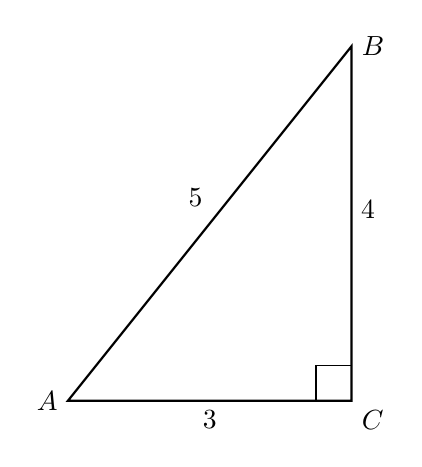
\begin{tikzpicture}[scale=0.9]
        \draw [thick]
        (0,0)node[left]{$A$}--
        (4,0)node[below right]{$C$}--
        (4,5)node[right]{$B$}--cycle;
        \draw (4,0)++(-0.5,0)--++(0,0.5)--+(0.5,0);
        \node at (2,0)[below]{$3$};
        \node at (4,2.7)[right]{$4$};
        \node at (1.8,2.6)[above]{$5$};
      \end{tikzpicture}
\end{flushright}
\end{multicols}

\item $\triangle ABC$ is shown with $m\angle C=90^\circ$. The lengths of the triangle's sides are $a$, $b$, and $c$. Express each trigonometric ratio as a fraction of two variables. \vspace{0.5cm}
\begin{multicols}{2}
    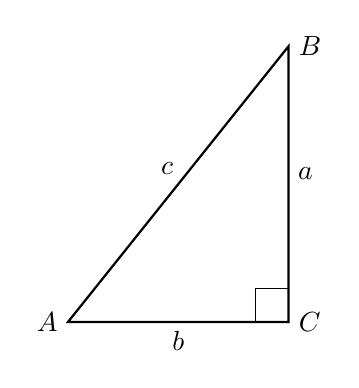
\begin{tikzpicture}[scale=0.7]
      \draw [thick]
      (0,0)node[left]{$A$}--
      (4,0)node[right]{$C$}--
      (4,5)node[right]{$B$}--cycle;
      \draw (4,0)++(-0.6,0)--++(0,0.6)--+(0.6,0);
      \node at (2,0)[below]{$b$};
      \node at (4,2.7)[right]{$a$};
      \node at (1.8,2.5)[above]{$c$};
    \end{tikzpicture}
      \begin{enumerate}
      \item $\sin A =$ \vspace{0.75cm}
      \item $\cos A =$ \vspace{0.75cm}
      \item $\tan A =$ \vspace{0.75cm}
    \end{enumerate}
\end{multicols}

\item Use the sine function to find the height $h$ of the right $\triangle ABC$ shown below.
  \begin{flushright}
    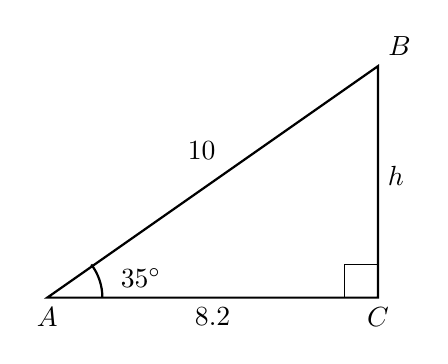
\begin{tikzpicture}[scale=0.7]
      \draw [thick](0,0)node[below]{$A$}--
      (6,0)node[below]{$C$}--
      (6,4.2)node[above right]{$B$}--cycle;
      \draw (6,0)++(-0.6,0)--++(0,0.6)--+(0.6,0);
      \node at (2.8,3)[below]{$10$};
      \node at (3,0)[below]{$8.2$};
      \node at (6,2.2)[right]{$h$};
      \draw [thick, -] (1,0) arc [start angle=0, end angle=37, radius=1];
      \node at (1.7,0)[above]{$35^\circ$};
    \end{tikzpicture}
  \end{flushright}
  Find the area of $\triangle ABC$ using the formula $A=\frac{1}{2}bh$

\newpage
\item Given $\triangle ABC$ with $AC=9$ centimeters, altitude $h=7$ cm, and the base $BC=13 \frac{1}{2}$ cm. \hfill \emph{diagram not to scale}
\begin{multicols}{2}
  \begin{enumerate}
    \item Write down $\sin C$ as a fraction.\\[0.5cm]
    $\sin C=$
    \item Find the area of $\triangle ABC$. \vspace{1.5cm}
  \end{enumerate}
  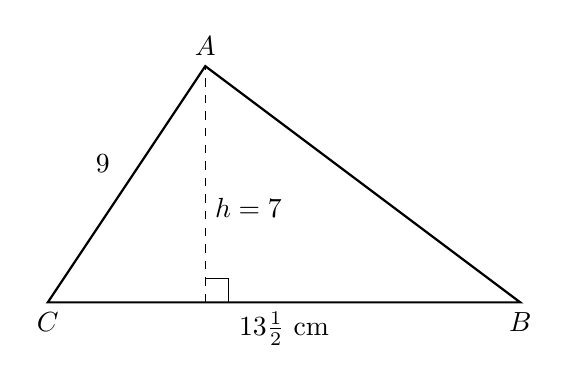
\begin{tikzpicture}[scale=1.]
    \draw [thick]
      (2,0)node[below]{$C$}--
      (8,0)node[below]{$B$}--
      (4,3)node[above]{$A$}--cycle;
   \draw [dashed] (4,0)--(4,3);
   \draw (4,0)++(0.3,0)--++(0,0.3)--+(-0.3,0);
   \node at (4,1.2)[right]{$h=7$};
   \node at (2.7,2)[below]{$9$};
   \node at (5,0)[below]{$13 \frac{1}{2}$ cm};
  \end{tikzpicture}  
\end{multicols} \vspace{1.5cm}

\item Two sides of $\triangle ABC$ are given $AC=10$ and $BC=12$, with the included angle m$\angle C=37^\circ$.
\begin{multicols}{2}
  \begin{enumerate}
    \item Find altitude $h$ using $\displaystyle \sin 37^\circ= \frac{h}{10}$.
    \item Find the area of $\triangle ABC$. \vspace{1.cm}
  \end{enumerate}
  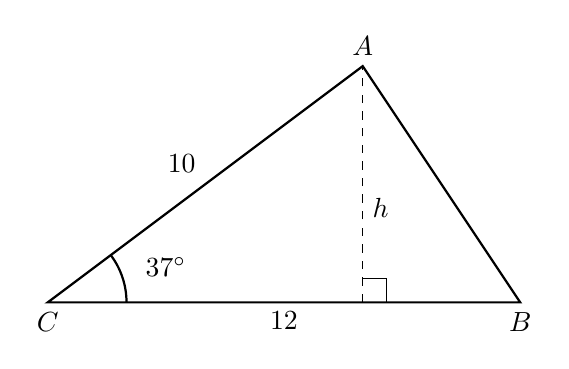
\begin{tikzpicture}[scale=1.]
    \draw [thick]
      (0,0)node[below]{$C$}--
      (6,0)node[below]{$B$}--
      (4,3)node[above]{$A$}--cycle;
   \draw [dashed] (4,0)--(4,3);
   \draw (4,0)++(0.3,0)--++(0,0.3)--+(-0.3,0);
   \draw [thick, -] (1,0) arc [start angle=0, end angle=37, radius=1];
   \node at (1.5,0.2)[above]{$37^\circ$};
   \node at (4,1.2)[right]{$h$};
   \node at (1.7,2)[below]{$10$};
   \node at (3,0)[below]{$12$};
  \end{tikzpicture}  
\end{multicols} \vspace{1cm}

\subsubsection*{Sine formula for the area of a triangle $\displaystyle A=\frac{1}{2}ab \sin C$}
\item Find the area of the given triangle.
\begin{flushright}
  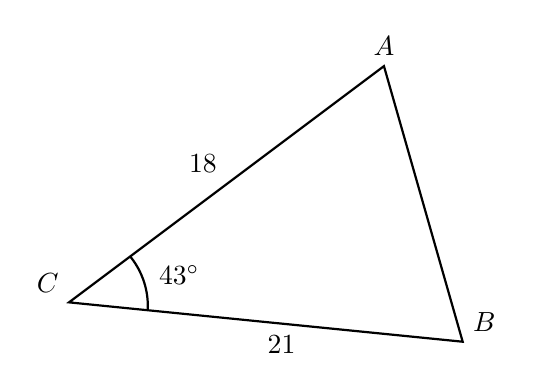
\begin{tikzpicture}[scale=1.]
    \draw [thick]
      (0,0)node[above left]{$C$}--
      (5,-0.5)node[above right]{$B$}--
      (4,3)node[above]{$A$}--cycle;
   \draw [thick, -] (1,-0.1) arc [start angle=-3, end angle=39, radius=1];
   \node at (1.4,0.1)[above]{$43^\circ$};
   \node at (1.7,2)[below]{$18$};
   \node at (2.7,-0.3)[below]{$21$};
  \end{tikzpicture}
\end{flushright}

\end{enumerate}
\end{document}
  